\documentclass[11pt,a4paper]{article}

% Packages
\usepackage[utf8]{inputenc}
\usepackage[T1]{fontenc}
% \usepackage{lmodern} % Removed - not installed
\usepackage[margin=1in]{geometry}
\usepackage{graphicx}
\graphicspath{{plots/}}
\usepackage{booktabs}
\usepackage{array}
\usepackage{longtable}
\usepackage{hyperref}
\usepackage{xcolor}
\usepackage{listings}
\usepackage{float}
\usepackage{amsmath}
\usepackage{amssymb}
\usepackage{tcolorbox}
\usepackage{enumitem}
\usepackage{fancyhdr}
\usepackage{titlesec}

% Colors
\definecolor{codegreen}{rgb}{0,0.6,0}
\definecolor{codegray}{rgb}{0.5,0.5,0.5}
\definecolor{codepurple}{rgb}{0.58,0,0.82}
\definecolor{backcolour}{rgb}{0.95,0.95,0.92}
\definecolor{anthropicblue}{RGB}{45,90,140}
\definecolor{warnorange}{RGB}{230,126,34}
\definecolor{successgreen}{RGB}{39,174,96}

% Code listing style
\lstdefinestyle{mystyle}{
    backgroundcolor=\color{backcolour},
    commentstyle=\color{codegreen},
    keywordstyle=\color{blue},
    numberstyle=\tiny\color{codegray},
    stringstyle=\color{codepurple},
    basicstyle=\ttfamily\footnotesize,
    breakatwhitespace=false,
    breaklines=true,
    captionpos=b,
    keepspaces=true,
    numbers=left,
    numbersep=5pt,
    showspaces=false,
    showstringspaces=false,
    showtabs=false,
    tabsize=2,
    frame=single,
    framerule=0pt,
}
\lstset{style=mystyle}

% Custom boxes
\newtcolorbox{keyinsight}{
    colback=anthropicblue!10,
    colframe=anthropicblue,
    title=\textbf{Key Insight},
    fonttitle=\bfseries
}

\newtcolorbox{warningbox}{
    colback=warnorange!10,
    colframe=warnorange,
    title=\textbf{Warning},
    fonttitle=\bfseries
}

\newtcolorbox{tipbox}{
    colback=successgreen!10,
    colframe=successgreen,
    title=\textbf{Tip},
    fonttitle=\bfseries
}

% Header/Footer
\pagestyle{fancy}
\fancyhf{}
\rhead{VLM Fine-Tuning Tutorial}
\lhead{InternVL3 on RoboVQA}
\rfoot{Page \thepage}

% Title formatting
\titleformat{\section}
    {\Large\bfseries\color{anthropicblue}}
    {\thesection}{1em}{}
\titleformat{\subsection}
    {\large\bfseries}
    {\thesubsection}{1em}{}

% Hyperref setup
\hypersetup{
    colorlinks=true,
    linkcolor=anthropicblue,
    filecolor=magenta,
    urlcolor=cyan,
    pdftitle={VLM Fine-Tuning Tutorial},
    pdfauthor={Giri},
}

\begin{document}

% Title Page
\begin{titlepage}
    \centering
    \vspace*{2cm}
    
    {\Huge\bfseries Vision-Language Model Fine-Tuning\\[0.5cm]}
    {\LARGE A Complete Practical Guide\\[1cm]}
    
    \vspace{1cm}
    
    {\Large\itshape From Zero to Training Your Own Robotics VLM\\[0.5cm]}
    {\large Fine-tuning InternVL3-8B on RoboVQA with Curriculum Learning}
    
    \vspace{2cm}
    
    \begin{tcolorbox}[colback=backcolour,colframe=codegray,width=0.8\textwidth]
    \centering
    \textbf{What You'll Learn:}
    \begin{itemize}[leftmargin=*]
        \item How Vision-Language Models process multimodal data
        \item QLoRA: Training 8B+ parameter models on consumer hardware
        \item Curriculum learning for robotics scene understanding
        \item Complete pipeline from raw data to trained model
        \item Real-world results and lessons learned
    \end{itemize}
    \end{tcolorbox}
    
    \vfill
    
    {\large January 2026}
    
\end{titlepage}

% Table of Contents
\tableofcontents
\newpage

%==========================================
\section{Introduction: What Are We Building?}
%==========================================

\subsection{The Goal}

We are fine-tuning \textbf{InternVL3-8B}, an 8-billion parameter Vision-Language Model, on the \textbf{RoboVQA dataset} to create a model that can understand robotics scenes and answer questions about them. Think of it as teaching an AI to look at robot camera footage and intelligently answer questions like:

\begin{itemize}
    \item ``What objects can the robot grasp?'' (Affordance detection)
    \item ``What should the robot do next to complete this task?'' (Planning)
    \item ``Did the robot successfully pick up the object?'' (Success prediction)
\end{itemize}

\subsection{Why This Matters}

Vision-Language Models (VLMs) represent the cutting edge of multimodal AI. They can process both images and text, understanding the relationship between what they see and what they're asked. For robotics, this capability is transformative---instead of hand-coding every visual pattern, we can train models to understand visual scenes naturally.

\subsection{VLMs vs VLAs: An Important Distinction}

\begin{keyinsight}
Before diving in, let's clarify a common confusion:
\begin{itemize}
    \item \textbf{VLM (Vision-Language Model)}: Understands images and generates text. Great for reasoning, planning, and understanding scenes.
    \item \textbf{VLA (Vision-Language-Action Model)}: Outputs actual robot control signals (joint positions, velocities, etc.).
\end{itemize}
Our fine-tuned VLM will NOT directly control a robot. Instead, it serves as a \textbf{reasoning module} in a larger system---understanding scenes and providing high-level guidance that other components translate into actions.
\end{keyinsight}

\subsection{Project Overview}

\begin{table}[H]
\centering
\begin{tabular}{@{}ll@{}}
\toprule
\textbf{Component} & \textbf{Choice} \\
\midrule
Base Model & InternVL3-8B \\
Dataset & RoboVQA (221,912 video samples) \\
Training Method & QLoRA (4-bit quantization + LoRA) \\
Training Strategy & Two-stage curriculum learning \\
Hardware & DGX Spark (GB10 Blackwell, 128GB) \\
Training Time & $\sim$25 days (Stage 1) + $\sim$22 days (Stage 2, including crash recovery) \\
\bottomrule
\end{tabular}
\caption{Project configuration summary}
\end{table}

%==========================================
\section{Understanding Vision-Language Models}
%==========================================

\subsection{The Architecture (Simplified)}

A VLM has three main components working together:

\begin{figure}[H]
\centering
\begin{tcolorbox}[colback=white,colframe=anthropicblue,width=\textwidth]
\begin{verbatim}
+-------------------+    +---------------------+    +-------------------+
|  Vision Encoder   | -> | Vision-Language     | -> |  Language Model   |
|  (InternViT-300M) |    | Connector (MLP)     |    |  (InternLM2.5-7B) |
+-------------------+    +---------------------+    +-------------------+
       ^                                                    |
    Images                                            Text Response
\end{verbatim}
\end{tcolorbox}
\caption{VLM architecture overview}
\end{figure}

\textbf{Vision Encoder}: Takes images and converts them into ``visual tokens''---numerical representations that capture what's in the image. InternVL3-8B uses InternViT-300M, which processes images at 448$\times$448 resolution.

\textbf{Vision-Language Connector}: A bridge (typically an MLP) that translates visual tokens into a format the language model understands. Think of it as a translator between ``image speak'' and ``text speak.''

\textbf{Language Model}: The brain of the operation. It takes the translated visual information plus your text prompt and generates a response. InternVL3-8B uses InternLM2.5-7B as its language backbone.

\subsection{How Images Become Tokens}

When you feed an image to InternVL3, the following transformation occurs:

\begin{enumerate}
    \item The image is resized to 448$\times$448 pixels
    \item It's divided into patches (like cutting a photo into a grid)
    \item Each patch becomes a token (typically 256 tokens per image)
    \item Multiple images = multiple sets of tokens
\end{enumerate}

For video data (like our robotics data with 16 frames):

\begin{equation}
\text{Visual Tokens} = \text{Frames} \times \text{Tokens per Frame} = 4 \times 256 = 1,024 \text{ tokens}
\end{equation}

\begin{warningbox}
This is critical for memory calculations---more frames = more tokens = more GPU memory. We use 4 frames in Stage 1 and 10 frames in Stage 2 to balance temporal context with memory constraints.
\end{warningbox}

\subsection{The Conversation Format}

VLMs are trained on conversations. Here's what a training sample looks like:

\begin{lstlisting}[language=Python,caption=Conversation format for VLM training]
{
  "conversations": [
    {
      "from": "human", 
      "value": "<image><image><image><image>Looking at these frames 
                from a robot camera, what objects can the robot reach?"
    },
    {
      "from": "gpt", 
      "value": "The robot can currently reach a red ball on the table 
                and a blue cup positioned to its right."
    }
  ]
}
\end{lstlisting}

The \texttt{<image>} tags are placeholders that get replaced with actual visual tokens during training. The model learns to associate visual patterns with the corresponding text responses.

%==========================================
\section{The Hardware Reality Check}
%==========================================

\subsection{Memory Requirements}

Training VLMs is memory-intensive. Here's a breakdown for InternVL3-8B:

\begin{table}[H]
\centering
\begin{tabular}{@{}lrr@{}}
\toprule
\textbf{Component} & \textbf{QLoRA} & \textbf{Full Fine-tune} \\
\midrule
Model weights & $\sim$5 GB (4-bit) & $\sim$16 GB (bfloat16) \\
LoRA adapters & $\sim$0.2 GB & N/A \\
Optimizer states & $\sim$0.3 GB & $\sim$32 GB \\
Gradients & $\sim$0.2 GB & $\sim$16 GB \\
Activations (4 frames) & $\sim$2--4 GB & $\sim$8--16 GB \\
\midrule
\textbf{Total} & \textbf{$\sim$10 GB} & \textbf{$\sim$72+ GB} \\
\bottomrule
\end{tabular}
\caption{Memory requirements comparison}
\end{table}

This is why we use QLoRA---it makes training possible on reasonable hardware.

\subsection{Our Setup: DGX Spark}

We trained on NVIDIA DGX Spark with:
\begin{itemize}
    \item \textbf{GPU}: GB10 Blackwell (128GB unified memory)
    \item \textbf{CUDA}: 13.0
    \item \textbf{Architecture}: sm\_121
\end{itemize}

The unified memory architecture shares memory between CPU and GPU, which changes some optimization strategies.

\subsection{Flash Attention on New Hardware: A Cautionary Tale}

\begin{keyinsight}
Cutting-edge hardware doesn't always work with cutting-edge software. Always benchmark!
\end{keyinsight}

We attempted to compile Flash Attention 2 for the GB10 (sm\_121), which required:
\begin{enumerate}
    \item Adding sm\_121 to the build configuration
    \item Updating CUTLASS to v4.3.0 for CUDA 13.0 compatibility
    \item Patching CUDA type definitions
    \item Modifying runtime architecture checks
\end{enumerate}

\textbf{Result}: It compiled and ran, but benchmarking revealed surprising results:

\begin{table}[H]
\centering
\begin{tabular}{@{}lr@{}}
\toprule
\textbf{Implementation} & \textbf{Latency (512 tokens)} \\
\midrule
Flash Attention 2 & 489ms \\
Flash Attention 3 & 489ms \\
\textbf{PyTorch SDPA} & \textbf{481ms} \\
\bottomrule
\end{tabular}
\caption{Attention implementation benchmarks on GB10}
\end{table}

SDPA was actually 2\% faster! The Flash Attention kernels weren't optimized for Blackwell's architecture. \textbf{Lesson}: Always benchmark; don't assume newer = better.

%==========================================
\section{Choosing Your Model}
%==========================================

\subsection{Model Evaluation}

We evaluated three candidates for video-based robotics VQA:

\begin{table}[H]
\centering
\begin{tabular}{@{}lccc@{}}
\toprule
\textbf{Model} & \textbf{Video Support} & \textbf{DGX Spark Support} & \textbf{Decision} \\
\midrule
PaliGemma 3B & Requires frame extraction & No official support & Rejected \\
Qwen2.5-VL-7B & Native video & Community only & Considered \\
InternVL3-8B & Native video & Official playbooks & \textbf{Selected} \\
\bottomrule
\end{tabular}
\caption{Model comparison for our use case}
\end{table}

\subsection{Why InternVL3-8B?}

Key factors that drove our decision:
\begin{enumerate}
    \item NVIDIA provides official fine-tuning playbooks for InternVL3 on their hardware
    \item Native multi-image input matches RoboVQA's 16-frame format
    \item Strong embodied AI benchmarks
    \item Well-documented QLoRA recipes
    \item 8B parameters fit comfortably with QLoRA in 128GB unified memory
\end{enumerate}

\subsection{Model Size Trade-offs}

Bigger isn't always better for robotics tasks:

\begin{itemize}
    \item \textbf{InternVL3-1B}: Fast inference, limited reasoning
    \item \textbf{InternVL3-2B}: Good balance for simple tasks
    \item \textbf{InternVL3-8B}: Strong reasoning, slower inference (our choice)
    \item \textbf{Larger models}: Diminishing returns for robotics tasks
\end{itemize}

For robotics VQA, we need enough capacity to understand complex spatial relationships but don't need the reasoning depth of a 70B model.

%==========================================
\section{Understanding Your Dataset: RoboVQA}
%==========================================

\subsection{Dataset Overview}

RoboVQA contains \textbf{221,912 video samples} of robot manipulation tasks. Each sample includes:
\begin{itemize}
    \item 16 frames of video at various resolutions
    \item Multiple QA pairs covering different aspects of the scene
    \item Task annotations categorizing each question type
\end{itemize}

\subsection{Task Type Distribution}

\begin{table}[H]
\centering
\begin{tabular}{@{}llr@{}}
\toprule
\textbf{Task Type} & \textbf{Description} & \textbf{Percentage} \\
\midrule
Affordance Detection & ``What can the robot interact with?'' & 33\% \\
Planning Variants & ``What should happen next?'' & 35\% \\
Success Prediction & ``Did the task succeed?'' & 14\% \\
Future Prediction & ``What will the scene look like?'' & 11\% \\
Past Description & ``What just happened?'' & 6\% \\
\bottomrule
\end{tabular}
\caption{RoboVQA task type distribution}
\end{table}

\subsection{The QA Text Format}

RoboVQA uses a structured format for its question-answer pairs:

\begin{lstlisting}[caption=RoboVQA text format]
<task:affordance:discriminative:discrete>
Looking at the scene, can the robot reach the red cup?
Q: Can the robot reach the red cup? A: Yes
\end{lstlisting}

The \texttt{<task:type:subtype:format>} marker tells us:
\begin{itemize}
    \item \textbf{type}: Main category (affordance, planning, etc.)
    \item \textbf{subtype}: Discriminative (yes/no) vs. generative (open-ended)
    \item \textbf{format}: Discrete answers vs. freeform text
\end{itemize}

This structure is important for preprocessing---we need to parse it correctly.

%==========================================
\section{Data Preprocessing: The Make-or-Break Step}
%==========================================

\subsection{Why Preprocessing Matters}

Raw data rarely matches what models expect. Poor preprocessing leads to:
\begin{itemize}
    \item Training failures (wrong format)
    \item Poor performance (information loss)
    \item Wasted compute (inefficient storage)
\end{itemize}

\subsection{Our Preprocessing Pipeline}

\begin{figure}[H]
\centering
\begin{tcolorbox}[colback=white,colframe=anthropicblue,width=\textwidth]
\begin{verbatim}
Raw TFRecords --> Frame Extraction --> JSONL Generation --> Ready for Training
     |                  |                    |
  221,912           3.5M JPEGs         Stage 1 & 2 splits
  videos            (~62GB)
\end{verbatim}
\end{tcolorbox}
\caption{Preprocessing pipeline overview}
\end{figure}

\subsection{Step 1: Frame Extraction}

\begin{lstlisting}[language=Python,caption=Frame extraction pseudocode]
for sample in tfrecord:
    for i, frame in enumerate(sample.frames):
        # Resize to model's expected size
        img = resize(frame, (448, 448))
        # Save with quality balance
        img.save(f"{unique_id}_{i:02d}.jpg", quality=85)
\end{lstlisting}

\begin{tipbox}
Key decisions for frame extraction:
\begin{itemize}
    \item \textbf{448$\times$448 resolution}: Matches InternVL3 input size
    \item \textbf{JPEG quality 85}: Good balance of size vs. quality
    \item \textbf{Shared image folder}: Both stages reference same images (saves $\sim$60GB)
\end{itemize}
\end{tipbox}

\subsection{Step 2: JSONL Format}

The training format follows InternVL conventions:

\begin{lstlisting}[language=Python,caption=JSONL training format]
{
  "id": "video_001_qa_0",
  "images": [
    "images/video_001_00.jpg",
    "images/video_001_01.jpg",
    "images/video_001_02.jpg",
    "images/video_001_03.jpg"
  ],
  "conversations": [
    {"from": "human", "value": "<image><image><image><image>What can the robot grasp?"},
    {"from": "gpt", "value": "The robot can grasp the red ball on the table."}
  ],
  "metadata": {"task_type": "affordance"}
}
\end{lstlisting}

\subsection{Stage 1 vs Stage 2 Format}

\textbf{Stage 1 (Visual Grounding)}: One QA pair per sample
\begin{lstlisting}[language=Python,caption=Stage 1 format: Single QA]
{
  "conversations": [
    {"from": "human", "value": "<image>...<image> Question 1?"},
    {"from": "gpt", "value": "Answer 1"}
  ]
}
\end{lstlisting}

\textbf{Stage 2 (Multi-Turn)}: All QAs from one video as conversation
\begin{lstlisting}[language=Python,caption=Stage 2 format: Multi-turn conversation]
{
  "conversations": [
    {"from": "human", "value": "<image>...<image> Question 1?"},
    {"from": "gpt", "value": "Answer 1"},
    {"from": "human", "value": "Question 2?"},
    {"from": "gpt", "value": "Answer 2"},
    {"from": "human", "value": "Question 3?"},
    {"from": "gpt", "value": "Answer 3"}
  ]
}
\end{lstlisting}

\subsection{Final Dataset Statistics}

\begin{table}[H]
\centering
\begin{tabular}{@{}llr@{}}
\toprule
\textbf{Stage} & \textbf{Split} & \textbf{Samples} \\
\midrule
Stage 1 & Train & 722,979 \\
Stage 1 & Validation & 80,330 \\
Stage 2 & Train & 199,721 \\
Stage 2 & Validation & 22,191 \\
\midrule
Images & & 3.5M JPEGs ($\sim$62GB) \\
\bottomrule
\end{tabular}
\caption{Final preprocessed dataset statistics}
\end{table}

%==========================================
\section{QLoRA: Training Large Models Efficiently}
%==========================================

\subsection{The Problem}

Full fine-tuning of an 8B model requires:
\begin{itemize}
    \item $\sim$16GB for model weights (bfloat16)
    \item $\sim$32GB for optimizer states (Adam stores 2 copies)
    \item $\sim$16GB for gradients
    \item Variable activation memory
\end{itemize}

\textbf{Total: 64GB+ just for basics}, before adding batch data.

\subsection{The Solution: QLoRA}

QLoRA combines three powerful techniques:

\subsubsection{4-bit Quantization}
Instead of 16 bits per parameter, we use 4 bits:
\begin{equation}
\text{Memory} = 8\text{B params} \times 4 \text{ bits} = 4\text{GB} \quad \text{(vs. 16GB for bfloat16)}
\end{equation}

\subsubsection{Low-Rank Adaptation (LoRA)}
Instead of updating all parameters, we add small ``adapter'' matrices:
\begin{equation}
\begin{aligned}
\text{Original}: \quad & W \in \mathbb{R}^{4096 \times 4096} = 16\text{M parameters} \\
\text{LoRA}: \quad & A \in \mathbb{R}^{4096 \times 128} + B \in \mathbb{R}^{128 \times 4096} = 1\text{M parameters}
\end{aligned}
\end{equation}

This is a \textbf{94\% reduction} in trainable parameters!

\subsubsection{Paged Optimizers}
Optimizer states are moved to CPU RAM when not needed, reducing GPU memory pressure.

\subsection{LoRA Configuration}

\begin{lstlisting}[language=Python,caption=LoRA configuration]
lora_r: 128        # Rank of adaptation matrices
lora_alpha: 256    # Scaling factor (typically 2x rank)
lora_dropout: 0.05 # Regularization
target_modules:    # Which layers to adapt
  - q_proj         # Query projection
  - k_proj         # Key projection  
  - v_proj         # Value projection
  - o_proj         # Output projection
  - gate_proj      # MLP gate
  - up_proj        # MLP up projection
  - down_proj      # MLP down projection
\end{lstlisting}

\subsection{Why These Target Modules?}

We adapt the \textbf{language model} attention and MLP layers because:
\begin{enumerate}
    \item They contain most of the learned knowledge
    \item Vision encoder benefits less from task-specific adaptation
    \item Connector is small enough to train directly if needed
\end{enumerate}

\subsection{Memory Savings Summary}

\begin{table}[H]
\centering
\begin{tabular}{@{}lr@{}}
\toprule
\textbf{Configuration} & \textbf{GPU Memory} \\
\midrule
Full fine-tune & 72+ GB \\
LoRA only & $\sim$24 GB \\
QLoRA & $\sim$10--12 GB \\
\bottomrule
\end{tabular}
\caption{Memory comparison across training methods}
\end{table}

QLoRA makes training possible on consumer GPUs (RTX 3090, RTX 4090) or workstations.

%==========================================
\section{Curriculum Learning: Why Order Matters}
%==========================================

\subsection{The Core Insight}

\begin{keyinsight}
Imagine teaching someone to write essays:
\begin{itemize}
    \item \textbf{Bad approach}: Give them complex essay prompts immediately
    \item \textbf{Good approach}: First teach sentences, then paragraphs, then essays
\end{itemize}
The same principle applies to VLM training.
\end{keyinsight}

\subsection{Our Two-Stage Curriculum}

\subsubsection{Stage 1: Visual Grounding (Foundation)}
\begin{itemize}
    \item One question-answer pair per video
    \item Teaches: Object recognition, spatial understanding, basic scene comprehension
    \item 722,979 training samples
    \item \textbf{Goal}: Model learns to ``see'' correctly
\end{itemize}

\subsubsection{Stage 2: Multi-Turn Reasoning (Advanced)}
\begin{itemize}
    \item Multiple QA pairs per video as conversation
    \item Teaches: Reasoning chains, task relationships, context maintenance
    \item 199,721 training samples
    \item Initialized from Stage 1 checkpoint
    \item \textbf{Goal}: Model learns to ``think'' about what it sees
\end{itemize}

\subsection{Why Not Skip Stage 1?}

We ran an ablation experiment to find out:

\begin{table}[H]
\centering
\begin{tabular}{@{}lccc@{}}
\toprule
\textbf{Training Approach} & \textbf{Stage 1 Eval Loss} & \textbf{Stage 2 Eval Loss} & \textbf{Difference} \\
\midrule
Curriculum (S1$\rightarrow$S2) & \textbf{0.334 / 1.40 ppl} & \textbf{0.034 / 1.03 ppl} & --- \\
Stage 2 Only & 0.495 / 1.64 ppl & 0.043 / 1.04 ppl & --- \\
\midrule
\textbf{Degradation} & \textbf{+48\% loss} & \textbf{+26\% loss} & \\
\bottomrule
\end{tabular}
\caption{Curriculum learning ablation results}
\end{table}

\begin{warningbox}
\textbf{Without Stage 1}: The model struggles with basic visual understanding, which cascades into worse reasoning performance.

\textbf{Conclusion}: The visual grounding stage is essential. You cannot build reasoning on a shaky visual foundation.
\end{warningbox}

\subsection{Stage Transition Strategy}

When moving from Stage 1 to Stage 2:

\begin{enumerate}
    \item \textbf{Load Stage 1 weights}: Start where we left off
    \item \textbf{Reset learning rate}: Fresh cosine schedule (but lower initial LR)
    \item \textbf{Reset best loss tracking}: Stage 2 metrics are different
    \item \textbf{Keep step counter}: For logging continuity
\end{enumerate}

\begin{lstlisting}[language=Python,caption=Stage 2 configuration]
# Stage 2 configuration
resume_from_checkpoint: experiments/stage1/checkpoints/final
reset_scheduler_on_resume: true  # Fresh LR schedule
learning_rate: 2.0e-5  # Lower than Stage 1's 4e-5
\end{lstlisting}

%==========================================
\section{The Training Pipeline}
%==========================================

\subsection{Project Structure}

\begin{lstlisting}[caption=Repository structure]
vlm-ft/
|-- vlmft/
|   |-- data/
|   |   |-- dataloader.py          # Dataset and collation
|   |   +-- preprocess_robovqa.py  # Raw data processing
|   |-- models/
|   |   +-- internvl.py            # Model loading and QLoRA setup
|   |-- training/
|   |   |-- trainer.py             # Training loop
|   |   +-- config.py              # Configuration dataclasses
|   +-- scripts/
|       |-- train.py               # Training entry point
|       +-- eval.py                # Evaluation entry point
|-- configs/
|   |-- stage1.yaml                # Stage 1 hyperparameters
|   |-- stage2.yaml                # Stage 2 hyperparameters
|   +-- stage2_only.yaml           # Ablation: skip Stage 1
+-- experiments/                   # Output directory
\end{lstlisting}

\subsection{The DataLoader}

\subsubsection{Dataset Class}
\begin{lstlisting}[language=Python,caption=Dataset implementation]
class RoboVQADataset(Dataset):
    def __getitem__(self, idx):
        sample = self.samples[idx]
        images = [Image.open(path) for path in sample["images"]]
        return {
            "images": images,
            "question": sample["conversations"][0]["value"],
            "answer": sample["conversations"][1]["value"],
        }
\end{lstlisting}

\subsubsection{Collator}
\begin{lstlisting}[language=Python,caption=Collator implementation]
class InternVLCollator:
    def __call__(self, batch):
        # Process images through model's vision preprocessing
        pixel_values = self.preprocess_images(batch)
        
        # Tokenize conversations
        input_ids, labels = self.tokenize_conversations(batch)
        
        # Create attention mask and image flags
        return {
            "pixel_values": pixel_values,
            "input_ids": input_ids,
            "attention_mask": attention_mask,
            "labels": labels,
            "image_flags": image_flags,
        }
\end{lstlisting}

\subsection{The Training Loop}

\begin{lstlisting}[language=Python,caption=Training loop pseudocode]
for epoch in range(num_epochs):
    for batch in train_dataloader:
        # Forward pass with mixed precision
        with torch.amp.autocast("cuda", dtype=torch.bfloat16):
            outputs = model(**batch)
            loss = outputs.loss / gradient_accumulation_steps
        
        # Backward pass
        loss.backward()
        
        # Update weights every N steps (gradient accumulation)
        if step % gradient_accumulation_steps == 0:
            torch.nn.utils.clip_grad_norm_(params, max_grad_norm)
            optimizer.step()
            scheduler.step()
            optimizer.zero_grad()
        
        # Periodic evaluation
        if step % eval_steps == 0:
            eval_metrics = evaluate(model, eval_dataloader)
            save_if_best(model, eval_metrics)
\end{lstlisting}

%==========================================
\section{Hyperparameters Explained}
%==========================================

\subsection{Complete Configuration}

\begin{table}[H]
\centering
\begin{tabular}{@{}llll@{}}
\toprule
\textbf{Parameter} & \textbf{Stage 1} & \textbf{Stage 2} & \textbf{Notes} \\
\midrule
LoRA rank (r) & 128 & 128 & InternVL official \\
LoRA alpha & 256 & 256 & 2$\times$r heuristic \\
LoRA dropout & 0.05 & 0.05 & --- \\
Learning rate & 4e-5 & 2e-5 & Lower for continued training \\
Batch size & 2 & 2 & Memory-optimized \\
Gradient accumulation & 16 & 16 & Effective batch: 32 \\
Epochs & 1 & 1 & Prevent overfitting \\
Warmup ratio & 0.03 & 0.03 & --- \\
LR scheduler & Cosine & Cosine & --- \\
Max grad norm & 1.0 & 1.0 & --- \\
Optimizer & AdamW & AdamW & $\beta_1$=0.9, $\beta_2$=0.999 \\
Weight decay & 0.01 & 0.01 & --- \\
Max frames & 4 & 10 & Memory vs. context \\
Max sequence length & 2048 & 4096 & Stage 2 needs longer \\
Attention & SDPA & SDPA & See Flash Attention section \\
Precision & bfloat16 & bfloat16 & Mixed precision \\
\bottomrule
\end{tabular}
\caption{Complete hyperparameter configuration}
\end{table}

\subsection{Key Hyperparameter Explanations}

\subsubsection{Batch Size and Gradient Accumulation}
\textbf{Problem}: We want large batch sizes for stable training, but GPU memory limits us to batch\_size=2.

\textbf{Solution}: Gradient accumulation simulates larger batches:
\begin{equation}
\text{Effective batch} = \text{batch\_size} \times \text{gradient\_accumulation\_steps} = 2 \times 16 = 32
\end{equation}

The model sees 32 samples before each weight update, but only 2 are in memory at once.

\subsubsection{Learning Rate}
\begin{itemize}
    \item \textbf{Stage 1}: Higher LR (4e-5) for initial learning
    \item \textbf{Stage 2}: Lower LR (2e-5) for refinement without catastrophic forgetting
\end{itemize}

\subsubsection{Learning Rate Schedule}

\begin{figure}[H]
\centering
\begin{tcolorbox}[colback=white,colframe=anthropicblue,width=0.8\textwidth]
\begin{verbatim}
LR
^
|   /~~~~~~~~~~~~~~~~\
|  /                  \
| /                    \
|/______________________\____
0    3%              100%    Steps
     Warmup  Cosine Decay
\end{verbatim}
\end{tcolorbox}
\caption{Learning rate schedule with warmup and cosine decay}
\end{figure}

\subsubsection{Sequence Length Calculation}
Memory calculation for Stage 1:
\begin{equation}
\text{Visual tokens} = 4 \text{ frames} \times 256 \text{ tokens/frame} = 1,024 \text{ tokens}
\end{equation}

We set max\_length=2048 to allow 1,024 visual + 1,024 text tokens.

%==========================================
\section{Engineering for Long-Running Training Jobs}
%==========================================

Training VLMs at scale is not just a machine learning problem---it's a \textit{systems engineering} problem. Our Stage 1 ran for 25 days and Stage 2 consumed over 22 days of compute (including crash recovery). During that time, we experienced two system crashes, lost days of compute, and learned hard lessons about what it takes to run training jobs that span weeks. This section distills those lessons.

\subsection{The Mindset Shift}

\begin{keyinsight}
When your training job runs for weeks, \textbf{everything that can go wrong will go wrong}. Power fluctuations, OS updates, memory spikes from edge-case samples, thermal events, WiFi drops causing NFS timeouts---you must design for failure from day one.
\end{keyinsight}

A 30-minute training job can afford sloppy engineering. A 30-day training job cannot. The discipline required is closer to running a production service than writing a research script.

\subsection{Checkpoint Strategy: The Most Important Decision}

\subsubsection{Our Costly Mistake}

We initially set \texttt{save\_steps: 5000} for Stage 2. With 227 seconds per step, that meant:

\begin{equation}
5000 \times 227\text{s} = 1{,}135{,}000\text{s} \approx \textbf{13.1 days between checkpoints}
\end{equation}

When the system crashed at step 27,186, our last checkpoint was at step 25,000. We lost \textbf{2,186 steps---roughly 6 days of compute}.

\begin{warningbox}
\textbf{The checkpoint frequency calculation}: Always convert \texttt{save\_steps} to wall-clock time. The formula is simple:

$\text{Time between saves} = \text{save\_steps} \times \text{seconds/step}$

If this number is greater than 24 hours, your checkpoint frequency is too low.
\end{warningbox}

\subsubsection{The Corrected Strategy}

After this painful lesson, we changed to \texttt{save\_steps: 500}:

\begin{equation}
500 \times 227\text{s} = 113{,}500\text{s} \approx \textbf{31 hours between checkpoints}
\end{equation}

When the system crashed again at step 28,929, our checkpoint at 28,500 meant we only lost \textbf{429 steps ($\sim$27 hours)}---still painful, but 5x better.

\begin{figure}[H]
\centering
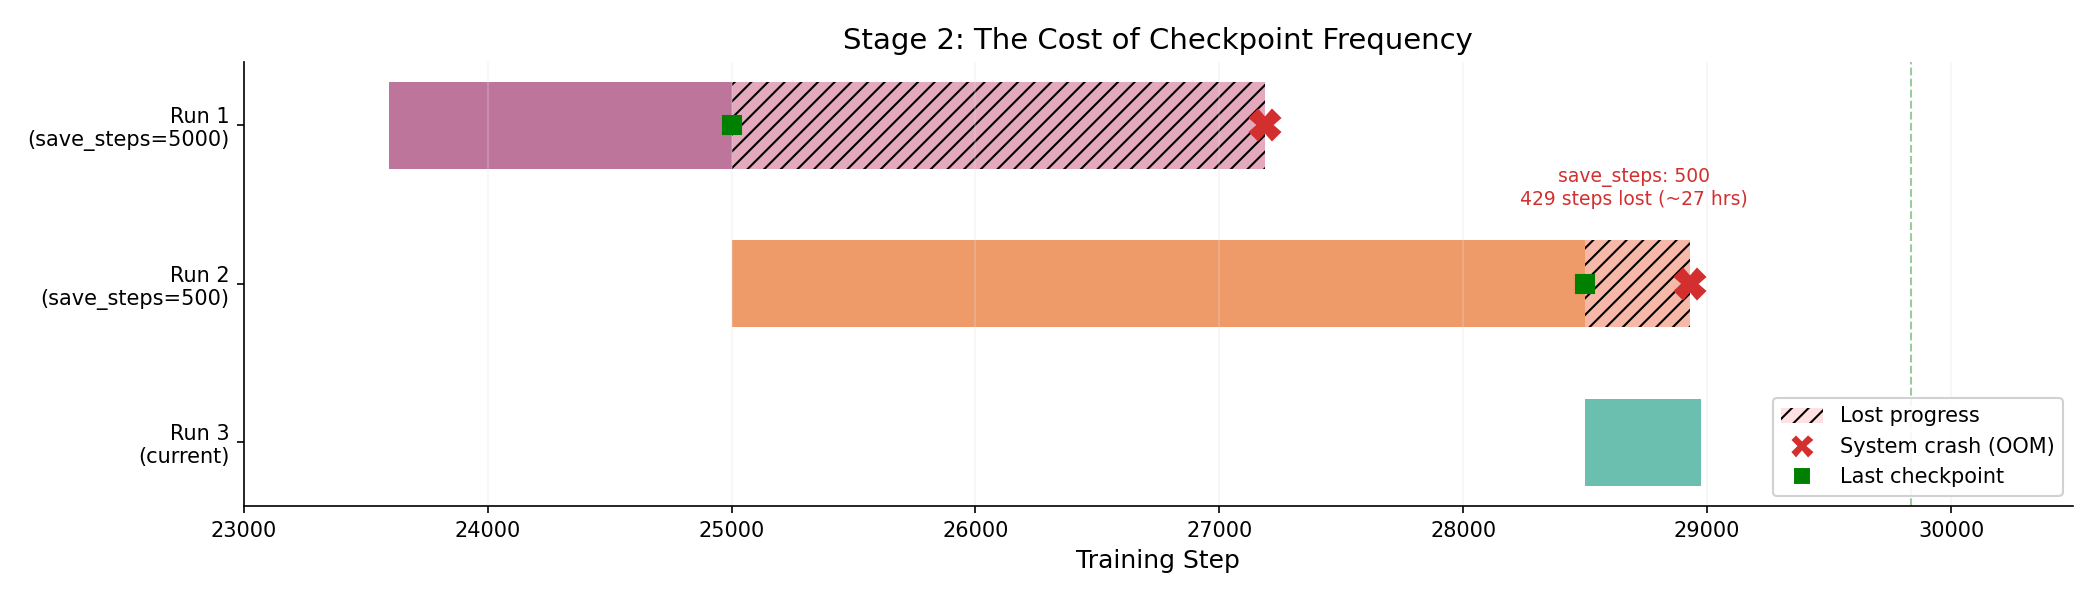
\includegraphics[width=\textwidth]{03_crash_recovery_timeline.png}
\caption{Stage 2 crash and recovery timeline. The hatched regions show lost progress---the difference between \texttt{save\_steps: 5000} (6 days lost) and \texttt{save\_steps: 500} (27 hours lost) is dramatic.}
\end{figure}

\subsubsection{Checkpoint Frequency Guidelines}

\begin{table}[H]
\centering
\begin{tabular}{@{}lll@{}}
\toprule
\textbf{Step Time} & \textbf{Recommended save\_steps} & \textbf{Time Between Saves} \\
\midrule
$<$ 10s & 2000--5000 & 6--14 hours \\
10--60s & 1000--2000 & 3--33 hours \\
60--120s & 500--1000 & 8--33 hours \\
$>$ 120s & 250--500 & 8--17 hours \\
\bottomrule
\end{tabular}
\caption{Checkpoint frequency recommendations by step time}
\end{table}

\textbf{Rule of thumb}: You should never lose more than 24 hours of compute to a crash. Disk space is cheap; GPU time is not.

\subsubsection{Checkpoint Retention}

Use \texttt{save\_total\_limit} to avoid filling your disk. Keep the 3--5 most recent checkpoints plus the best checkpoint based on eval loss. Our directory structure:

\begin{lstlisting}[caption=Checkpoint directory]
checkpoints/
  step_27500/    # Recent
  step_28000/    # Recent  
  step_28500/    # Most recent
  best/          # Symlink to best eval loss checkpoint
  final/         # Saved at end of training
\end{lstlisting}

\subsubsection{Always Save on Completion}

Our Stage 1 saved checkpoints every 1000 steps, but training ran for 2,259 steps. The final checkpoint was at step 2000---missing the last 259 steps. Always force a save at training completion, regardless of the step interval.

%==========================================
\section{Monitoring and Observability}
%==========================================

\subsection{Integrated Profiling: Not Optional}

We built timing instrumentation directly into the training loop, logging every metric to CSV files. This proved invaluable for diagnosing issues weeks into training.

\subsubsection{Per-Step Timing Metrics}

\begin{lstlisting}[language=Python,caption=Profiling instrumentation in the training loop]
# Timing every phase of each training step
t_start = time.time()

# 1. Data loading
t0 = time.time()
batch = next(data_iter)
t_data = time.time() - t0

# 2. CPU -> GPU transfer
t0 = time.time()
batch = to_device(batch)
t_transfer = time.time() - t0

# 3. Forward pass
t0 = time.time()
loss = model(**batch).loss
t_forward = time.time() - t0

# 4. Backward pass
t0 = time.time()
loss.backward()
t_backward = time.time() - t0

# 5. Optimizer step (every N accumulation steps)
t0 = time.time()
optimizer.step()
t_optimizer = time.time() - t0

t_step = time.time() - t_start
throughput = batch_size / t_step
gpu_mem = torch.cuda.memory_allocated() / 1e9
\end{lstlisting}

\subsubsection{What Each Metric Tells You}

\begin{table}[H]
\centering
\begin{tabular}{@{}p{2.5cm}p{4cm}p{6cm}@{}}
\toprule
\textbf{Metric} & \textbf{Healthy Signal} & \textbf{Problem Indicators} \\
\midrule
\texttt{t\_data} & $<$ 0.1s (negligible) & $>$ 1s: I/O bottleneck, slow disk, few workers \\
\texttt{t\_transfer} & $<$ 0.1s (negligible) & $>$ 0.5s: Large batch or memory pressure \\
\texttt{t\_forward} & Consistent & Spikes: variable-length sequences hitting max \\
\texttt{t\_backward} & $\sim$1.5--2$\times$ forward & $>$3$\times$ forward: gradient checkpointing issue \\
\texttt{t\_optimizer} & $<$ 0.5s & Spikes: paged optimizer swapping to CPU \\
\texttt{gpu\_mem\_gb} & Stable & Growing: memory leak; spiking: OOM risk \\
\texttt{throughput} & Consistent & Declining: thermal throttling or background load \\
\bottomrule
\end{tabular}
\caption{Per-step profiling metrics interpretation}
\end{table}

\begin{figure}[H]
\centering
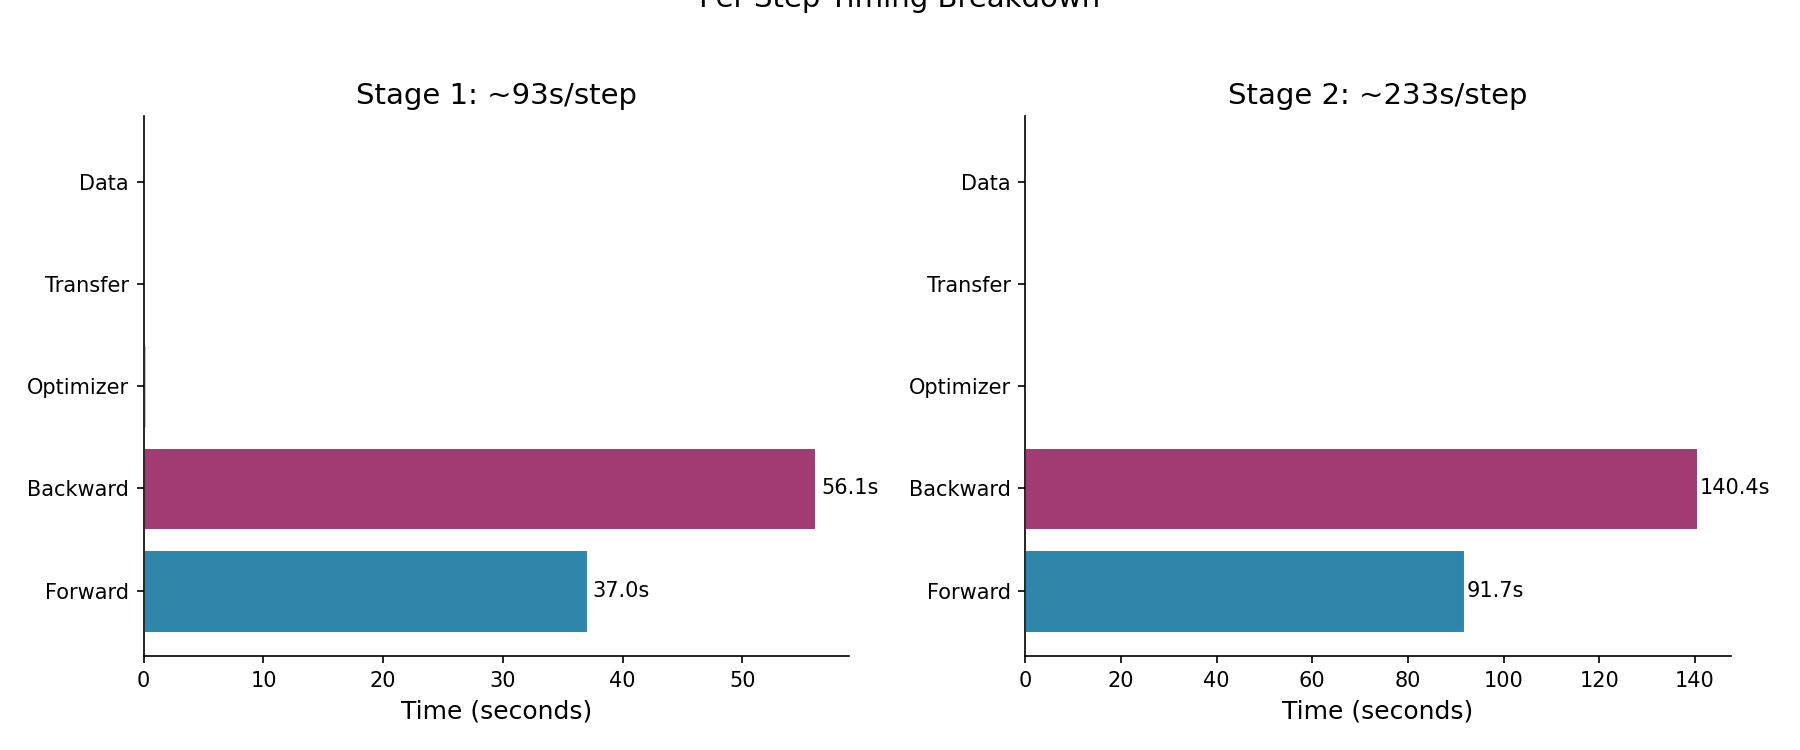
\includegraphics[width=\textwidth]{06_timing_breakdown.png}
\caption{Per-step timing breakdown for Stage 1 vs Stage 2. The backward pass dominates in both stages ($\sim$60\% of step time). Stage 2 steps take $\sim$2.5$\times$ longer due to longer sequences and more frames.}
\end{figure}

\subsubsection{CSV Logging}

Every metric is appended to a CSV file on every step:

\begin{lstlisting}[caption=Sample training CSV output]
step,loss,learning_rate,t_data,t_transfer,t_forward,t_backward,
  t_optimizer,t_step,throughput,gpu_mem_gb,timestamp
1000,0.234,3.92e-05,0.003,0.048,37.5,58.1,0.135,95.8,0.334,
  11.9,2025-12-10T14:23:01
\end{lstlisting}

This data is essential for post-hoc analysis. When a crash happens at 3 AM, you can look at the CSV to see whether step times were increasing, memory was growing, or throughput was declining before the crash.

\subsection{Key Health Indicators}

\begin{table}[H]
\centering
\begin{tabular}{@{}lll@{}}
\toprule
\textbf{Metric} & \textbf{Healthy Range} & \textbf{Warning Signs} \\
\midrule
Training loss & Decreasing & Sudden spikes, NaN, plateau \\
Eval loss & Decreasing & Increasing (overfitting) \\
Perplexity & $<$ 2.0 & $>$ 5.0 indicates problems \\
Learning rate & Following schedule & Stuck at 0 or not decaying \\
GPU memory & Stable & Growing or spiking \\
Step time & Consistent ($\pm$5\%) & Sudden increases \\
\bottomrule
\end{tabular}
\caption{Training health indicators}
\end{table}

\begin{figure}[H]
\centering
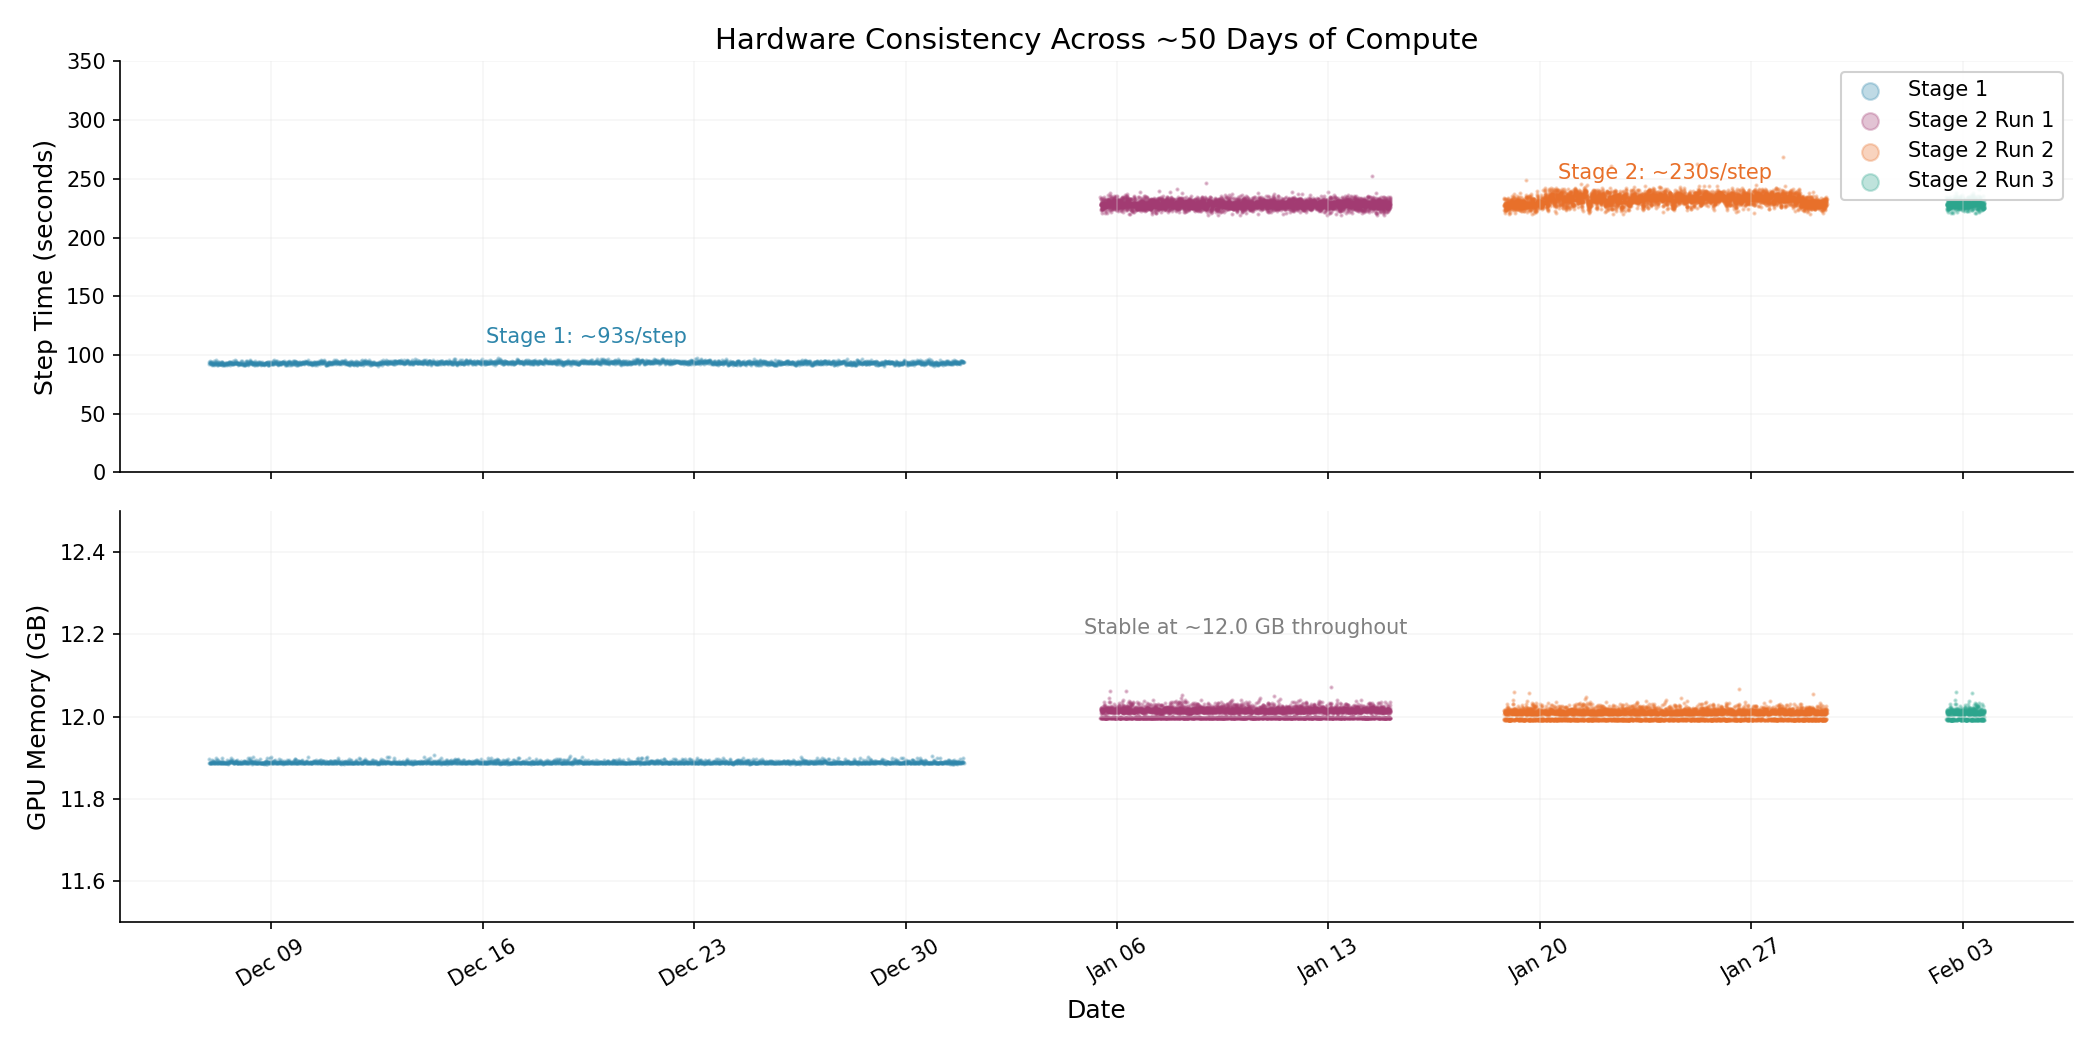
\includegraphics[width=\textwidth]{04_step_time_gpu_memory.png}
\caption{Step time and GPU memory over the entire training run. Both metrics remain remarkably stable throughout, confirming the crashes were caused by occasional memory spikes on extreme samples rather than gradual degradation.}
\end{figure}

\subsection{Verify Checkpoint Loading}

\begin{warningbox}
When resuming from a checkpoint, many training frameworks will \textbf{silently start from scratch} if the checkpoint path is invalid. Without explicit verification, you could waste hours of compute before noticing.
\end{warningbox}

Always log checkpoint loading explicitly and sanity-check the first step:

\begin{lstlisting}[language=Python,caption=Checkpoint loading verification]
def _load_checkpoint(self, path):
    # Load adapter weights
    adapter_state = load_file(path / "adapter_model.safetensors")
    set_peft_model_state_dict(self.model, adapter_state)
    logger.info(f"Loaded adapter weights from {path}")
    
    # Load training state
    state = torch.load(path / "training_state.pt")
    self.global_step = state["global_step"]
    logger.info(f"Resumed from checkpoint: step={self.global_step}")
    
    # CRITICAL: Verify loss is consistent with pre-crash
    # If step 1 loss is >> expected, checkpoint didn't load!
\end{lstlisting}

\textbf{The sanity check}: If your model was at loss 0.01 before the crash and step 1 after restart shows loss 1.26, the checkpoint didn't load. Catching this in the first few minutes saves hours of wasted compute.

\subsection{Automated Health Monitoring}

On a cluster, the job scheduler monitors your training and restarts on failure. On a single machine, crashes can go undetected for hours---until you happen to check in.

\begin{keyinsight}
A simple watchdog process that runs every 15--30 minutes can detect training failures within minutes and send notifications. This is trivial to set up and could save days over a multi-week run.
\end{keyinsight}

\begin{lstlisting}[language=bash,caption=Simple training watchdog (run via cron)]
#!/bin/bash
# Check if training is still running
if ! pgrep -f "train.py" > /dev/null; then
    LAST_STEP=$(tail -1 /path/to/train_metrics.csv)
    curl -X POST "$SLACK_WEBHOOK" \
      -d "{\"text\":\"Training stopped! Last: $LAST_STEP\"}"
fi
\end{lstlisting}

More sophisticated monitoring can track metric trends---alert if GPU memory is climbing, step time is increasing, or loss has gone to NaN---giving you early warning before a crash occurs.

\textbf{Rule}: If you're not monitoring it, you're not running it.

%==========================================
\section{Debugging Crashes on New Hardware}
%==========================================

\subsection{Our Crash Pattern}

During Stage 2 training, we experienced three system-level crashes that required hard reboots. The pattern was telling:

\begin{table}[H]
\centering
\begin{tabular}{@{}lrrll@{}}
\toprule
\textbf{Crash} & \textbf{Stopped At} & \textbf{Steps Lost} & \textbf{Root Cause} & \textbf{How Found} \\
\midrule
1st & Step 27,186 & 2,186 & GPU OOM & kern.log \\
2nd & Step 28,929 & 429 & GPU OOM & Inferred \\
\bottomrule
\end{tabular}
\caption{Stage 2 crash history}
\end{table}

\textbf{Key observation}: Stage 1 ran for 25 days with \textbf{zero crashes}. All crashes occurred during Stage 2. The difference? Stage 2 uses 2.5$\times$ longer sequences and more frames, creating occasional memory spikes.

\subsection{System Diagnostic Tools}

\subsubsection{dmesg: The First Check (But Often Useless)}

After a crash requiring reboot, \texttt{dmesg} shows the \textit{current} boot's messages, not the crash that caused the reboot:

\begin{lstlisting}[language=bash,caption=dmesg after reboot - only shows current boot]
$ dmesg | tail -20
# Shows current boot messages, NOT the crash
# nvidia-modeset errors here are display-related, NOT training OOM!
\end{lstlisting}

\begin{warningbox}
\texttt{nvidia-modeset: ERROR: Failed to allocate KBPS Iso} errors in \texttt{dmesg} are about \textbf{display output bandwidth}, not GPU compute memory. Do not confuse these with training OOMs---they are a red herring.
\end{warningbox}

\subsubsection{journalctl: Find Previous Boot Logs}

The real diagnostic gold is in the previous boot's logs:

\begin{lstlisting}[language=bash,caption=Using journalctl to find crash evidence]
# List all boots (previous boots have negative indices)
$ journalctl --list-boots
 -1 b7526ca7  Thu 2026-01-15 ... Thu 2026-01-29  # Previous
  0 376d6ae2  Mon 2026-02-02 ... Mon 2026-02-02  # Current

# Check previous boot's kernel messages
$ journalctl -b -1 -k | grep -i "oom\|error\|fail\|nvrm"
\end{lstlisting}

\subsubsection{Kernel Logs: The Smoking Gun}

This is how we found our root cause. In \texttt{/var/log/kern.log.1} (the previous boot's kernel log):

\begin{lstlisting}[caption=The GPU OOM evidence from kernel logs]
2026-01-28T14:34:16 NVRM: Check failed: Out of memory 
  [NV_ERR_NO_MEMORY] @ mem_desc.c:1359
2026-01-28T14:35:06 fill_page_cache_func hogged CPU 
  for >20000us 4 times
2026-01-28T14:36:19 NVRM: Out of memory (3 more times)
2026-01-28T14:36:44 NVRM: Out of memory (2 more times)
\end{lstlisting}

\textbf{The story}: The NVIDIA driver ran out of memory, the CPU started thrashing trying to handle the memory pressure (\texttt{fill\_page\_cache\_func hogged CPU}), and the system eventually became unresponsive---requiring a hard reboot.

\subsubsection{Thermal Monitoring}

\begin{lstlisting}[language=bash,caption=Monitoring GPU thermals]
# Check thermal zones (values in millidegrees Celsius)
$ cat /sys/class/thermal/thermal_zone*/temp
79500    # 79.5C - warm but safe
69800    # 69.8C
70700    # 70.7C

# Continuous monitoring during training
$ watch -n 1 'cat /sys/class/thermal/thermal_zone*/temp'
\end{lstlisting}

For sustained GPU training, temperatures below 85\textdegree C are safe. Throttling typically starts at 85--90\textdegree C. In our case, thermals were \textbf{not} the issue---confirmed by monitoring showing 79.5\textdegree C peak.

\subsection{The Root Cause: Unified Memory and Variable-Length Sequences}

\subsubsection{Why Stage 2 Crashed But Stage 1 Didn't}

\begin{table}[H]
\centering
\begin{tabular}{@{}lrr@{}}
\toprule
\textbf{Parameter} & \textbf{Stage 1} & \textbf{Stage 2} \\
\midrule
max\_frames & 4 & 10 \\
max\_length & 2048 & 4096 \\
Eval batch size & 8 & 4 (reduced from 8) \\
Step time & $\sim$93s & $\sim$230s \\
\bottomrule
\end{tabular}
\caption{Stage 1 vs Stage 2 memory pressure comparison}
\end{table}

Stage 2's longer sequences occasionally spike memory beyond what the system can handle. On the DGX Spark's unified memory architecture (128GB shared between CPU and GPU), there is no separate swap space---when GPU memory fills up, the entire system hangs rather than producing a clean CUDA OOM error.

\subsubsection{The Eval Batch Size Trap}

\begin{keyinsight}
The first crash occurred during evaluation, not training. Our eval batch size was 4 (2$\times$ training batch size). Combined with Stage 2's longer sequences, eval created larger memory spikes than training. This is easy to overlook because eval doesn't use gradients---but it processes more samples simultaneously.
\end{keyinsight}

\textbf{Fix}: Set eval batch size $\leq$ training batch size, especially for long-sequence stages.

\subsubsection{Memory Headroom}

We initially set \texttt{max\_memory\_gb: 115} on a 128GB system (90\% utilization). This left only 13GB of headroom---not enough for worst-case samples. After identifying the OOM pattern, we reduced to \texttt{max\_memory\_gb: 100} (78\% utilization), giving 28GB of headroom.

\textbf{Rule of thumb for unified memory systems}: Leave at least 20\% headroom. Variable-length sequences create unpredictable memory spikes.

\subsection{Debugging Tensor Mismatches and NaN Losses}

During our initial Stage 2 launch, we encountered NaN losses caused by a tensor shape mismatch:

\begin{lstlisting}[caption=The NaN-causing tensor mismatch warning]
warning: The size of tensor a (4081) must match the size of 
  tensor b (8192), input_embeds[selected].shape=
  torch.Size([4081, 3584]), vit_embeds.shape=
  torch.Size([8192, 3584])
\end{lstlisting}

\textbf{Root cause}: With \texttt{max\_frames=16}, visual tokens alone consumed 4,096 tokens ($16 \times 256$)---exactly equal to \texttt{max\_length=4096}. After adding conversation text, sequences were truncated, cutting off image placeholder tokens. The vision encoder produced embeddings for all 16 frames, but the text contained slots for fewer---a mismatch that produced NaN gradients.

\textbf{Fix}: Reduced \texttt{max\_frames} from 16 to 10, ensuring sufficient token budget for both visual and text content:

\begin{equation}
10 \text{ frames} \times 256 \text{ tokens/frame} = 2{,}560 \text{ visual tokens} + 1{,}536 \text{ for text} = 4{,}096
\end{equation}

\begin{warningbox}
\textbf{Always verify}: $(\text{max\_frames} \times \text{tokens/frame}) + \text{max text length} \leq \text{max\_length}$. Truncation of image placeholder tokens causes silent but catastrophic mismatches.
\end{warningbox}

%==========================================
\section{Evaluation and Validation}
%==========================================

\subsection{10\% Subset Validation}

Before full-scale training, we validated the pipeline on 10\% of the data:

\begin{table}[H]
\centering
\begin{tabular}{@{}lrrr@{}}
\toprule
\textbf{Stage} & \textbf{Eval Loss} & \textbf{Perplexity} & \textbf{Training Time} \\
\midrule
Stage 1 & 0.284 & 1.329 & $\sim$2.4 days \\
Stage 2 & 0.034 & 1.034 & $\sim$1.8 days \\
\bottomrule
\end{tabular}
\caption{10\% subset validation results}
\end{table}

\textbf{Observations}:
\begin{itemize}
    \item Consistent improvement throughout Stage 1 with no overfitting
    \item Stage 2 perplexity near 1.0 indicates high confidence on multi-turn reasoning
    \item Eval loss decreased monotonically, suggesting the model could benefit from more data
\end{itemize}

\subsection{Full-Scale Results}

\subsubsection{Stage 1: Visual Grounding (100\% Data)}

\begin{table}[H]
\centering
\begin{tabular}{@{}lrrr@{}}
\toprule
\textbf{Metric} & \textbf{10\% Run} & \textbf{Full Run} & \textbf{Improvement} \\
\midrule
Eval Loss & 0.284 & \textbf{0.125} & \textbf{56\% better} \\
Perplexity & 1.329 & \textbf{1.133} & --- \\
Training Steps & 2,259 & 22,593 & --- \\
Training Time & $\sim$2.4 days & $\sim$25 days & --- \\
\bottomrule
\end{tabular}
\caption{Stage 1 full training results}
\end{table}

\textbf{Training dynamics}:
\begin{itemize}
    \item Eval loss decreased monotonically from 0.322 $\rightarrow$ 0.125 with no plateau
    \item Step time: $\sim$93s (consistent throughout)
    \item GPU memory: 11.9 GB (stable)
    \item Model continued learning throughout without overfitting
\end{itemize}

\begin{keyinsight}
The full dataset delivered substantial gains over the 10\% validation run, confirming that the model benefits from more unique samples rather than multiple epochs over less data.
\end{keyinsight}

\begin{figure}[H]
\centering
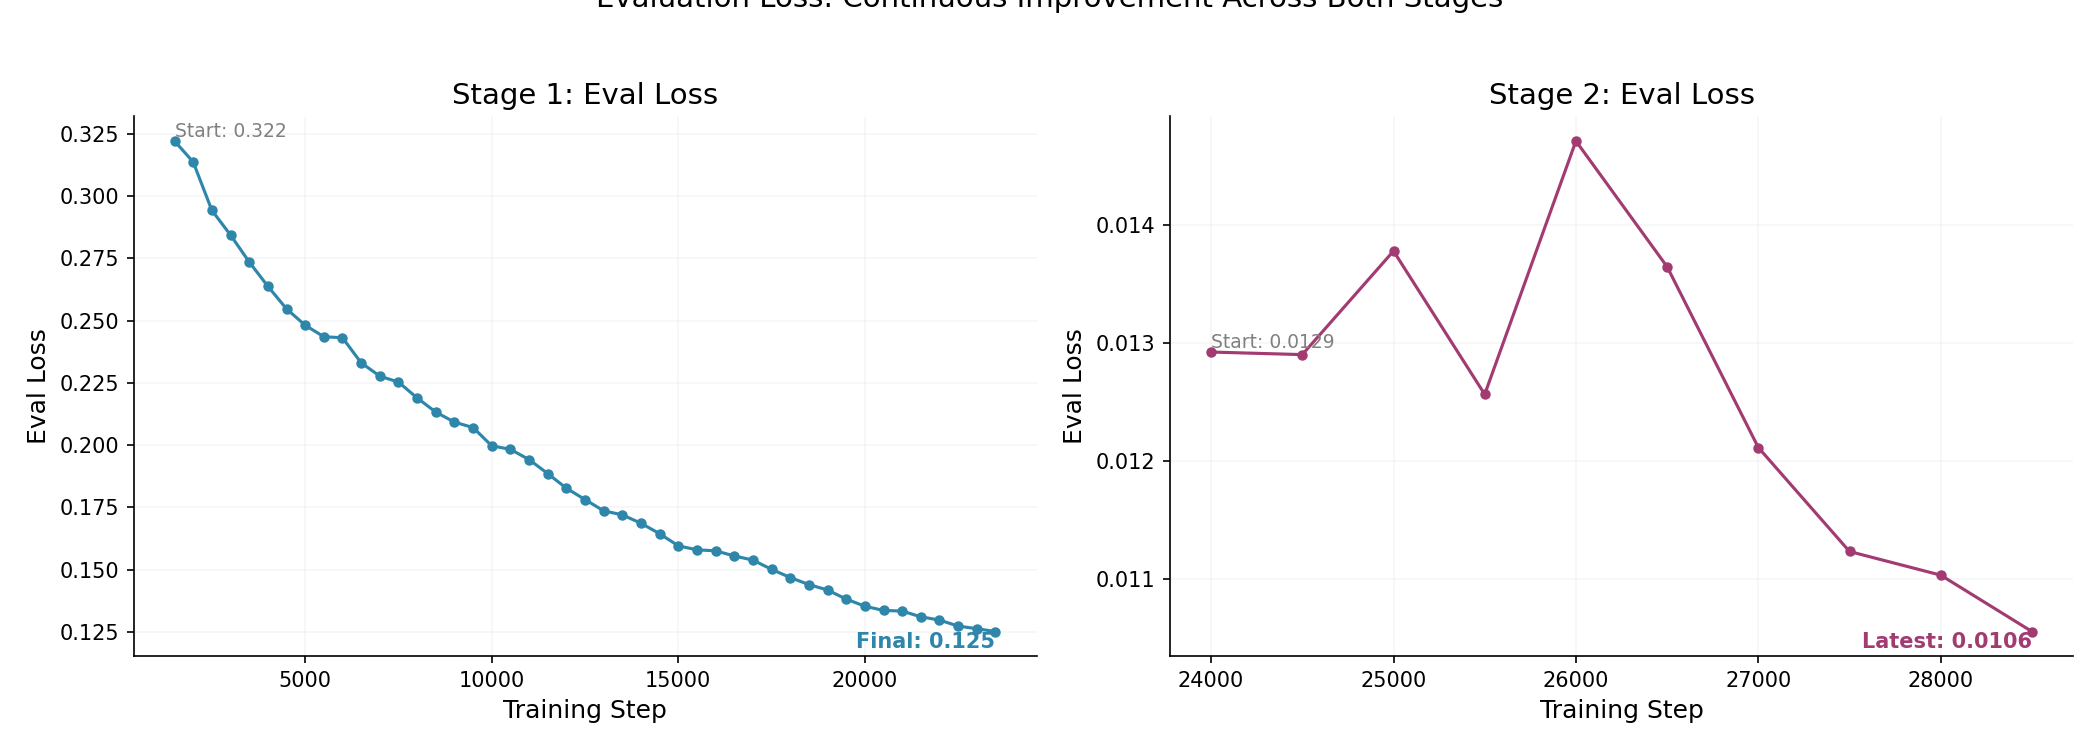
\includegraphics[width=\textwidth]{02_eval_loss_trajectory.png}
\caption{Evaluation loss over training steps. Stage 1 (left) shows steady improvement from 0.322 to 0.125 over 23K steps. Stage 2 (right) continues improving, with eval loss reaching 0.0106 and still decreasing.}
\end{figure}

%==========================================
\section{Battle-Tested Pitfalls and How to Avoid Them}
%==========================================

These are not hypothetical---every item below cost us hours or days of compute.

\subsection{Data Preprocessing Pitfalls}

\begin{enumerate}
    \item \textbf{Wrong image size}: We initially preprocessed at 288$\times$448, requiring expensive BICUBIC resize on every batch. Pre-resizing to 448$\times$448 during preprocessing and switching to BILINEAR interpolation for any remaining resizes dramatically improved data loading.
    \item \textbf{Missing image tokens}: If \texttt{<image>} count doesn't match actual images, InternVL produces tensor mismatches. Some multi-turn Stage 2 samples had image markers only in the first turn---the collator must handle this.
    \item \textbf{Token budget overflow}: With 16 frames $\times$ 256 tokens = 4,096 image tokens and \texttt{max\_length=4096}, zero budget remained for text. Truncation silently removed image placeholders, causing NaN losses.
    \item \textbf{Data leakage}: Keep train/val splits consistent across stages. Both stages should split on the same video IDs.
\end{enumerate}

\subsection{Checkpoint and Recovery Pitfalls}

\begin{enumerate}
    \item \textbf{save\_steps too large}: 5,000 steps at 227s/step = 13 days between checkpoints. One crash cost us 6 days.
    \item \textbf{No final checkpoint}: Training at 2,259 steps with \texttt{save\_steps: 1000} means the last save was at step 2,000---missing 259 steps. Always save on completion.
    \item \textbf{Silent restart on bad checkpoint path}: Many frameworks silently start from scratch if the path is invalid. Always verify by checking the first step's loss matches expectations.
    \item \textbf{Not saving optimizer/scheduler state}: Without optimizer state, resumed training uses a fresh optimizer, causing training instability. Without scheduler state, learning rate resets to warmup.
    \item \textbf{No failure monitoring}: Without a watchdog, crashes go undetected for hours. A simple cron job checking process liveness can alert you within minutes.
\end{enumerate}

\subsection{Memory and Stability Pitfalls}

\begin{enumerate}
    \item \textbf{Eval batch size larger than train}: We used eval\_batch\_size=4 with train\_batch\_size=2. Eval doesn't store gradients but processes 2$\times$ more samples simultaneously---this caused our first OOM crash.
    \item \textbf{Insufficient memory headroom}: 90\% utilization (115/128GB) left no room for worst-case samples. 78\% (100/128GB) proved stable.
    \item \textbf{Unified memory hangs instead of OOMing}: On DGX Spark, GPU OOM causes system freeze, not a Python exception. The only evidence is in kernel logs from the previous boot.
    \item \textbf{Assuming Flash Attention works}: We spent days compiling FA2 for Blackwell (sm\_121). It ran 2\% \textit{slower} than SDPA. Always benchmark.
\end{enumerate}

\subsection{Stage Transition Pitfalls}

\begin{enumerate}
    \item \textbf{Not resetting the LR scheduler}: When transitioning from Stage 1 to Stage 2, load weights but use a fresh cosine schedule. Otherwise, the learning rate continues decaying from Stage 1's end---near zero.
    \item \textbf{Not resetting best\_eval\_loss}: Stage 2's loss scale differs from Stage 1. Keep the old best loss and you'll never save a ``best'' checkpoint.
    \item \textbf{Wrong ``best'' checkpoint}: ``Best'' is based on eval loss, which may not correspond to the last checkpoint. Verify what ``best'' actually points to.
\end{enumerate}

%==========================================
\section{Results and Lessons Learned}
%==========================================

\subsection{Final Results Summary}

\begin{table}[H]
\centering
\begin{tabular}{@{}lrr@{}}
\toprule
\textbf{Metric} & \textbf{Stage 1 Final} & \textbf{Stage 2 Final} \\
\midrule
Eval Loss & 0.125 & (In progress) \\
Perplexity & 1.133 & (In progress) \\
Training Time & 25 days & $\sim$22 days \\
\bottomrule
\end{tabular}
\caption{Final training results}
\end{table}

\begin{figure}[H]
\centering
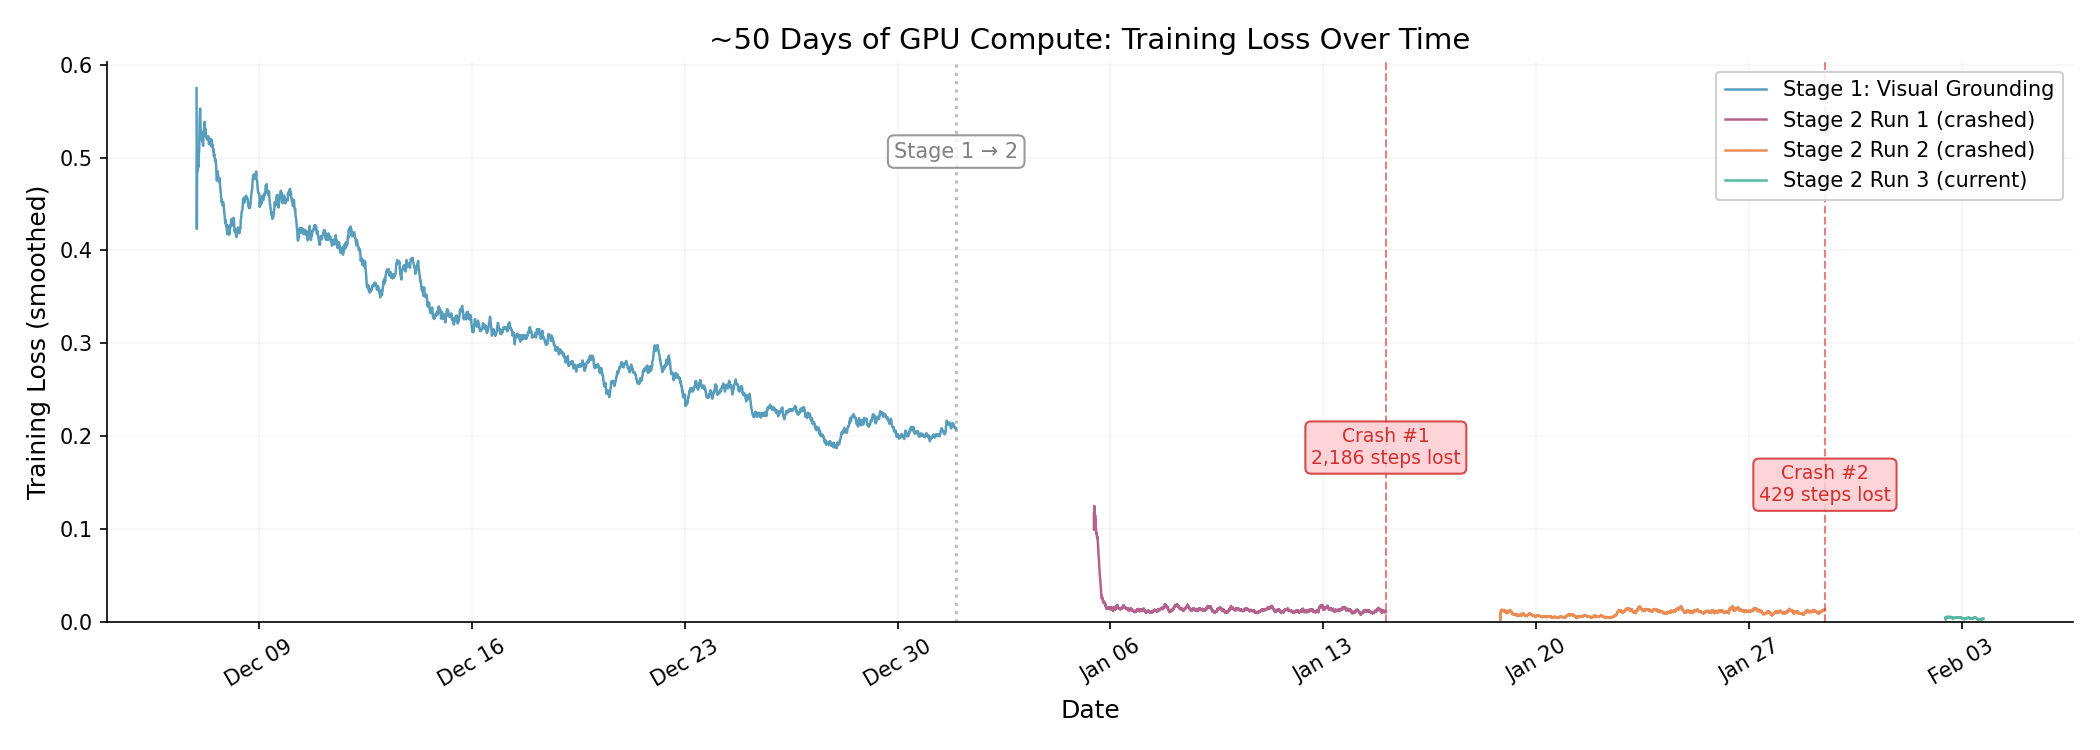
\includegraphics[width=\textwidth]{01_training_journey_timeline.png}
\caption{The complete training journey by calendar date, spanning Dec 6, 2025 to Feb 3, 2026. Stage 1 shows steady loss descent over 25 days. Stage 2 runs at much lower loss but suffered two OOM crashes (red dashed lines), requiring restarts from the last checkpoint.}
\end{figure}

\begin{figure}[H]
\centering
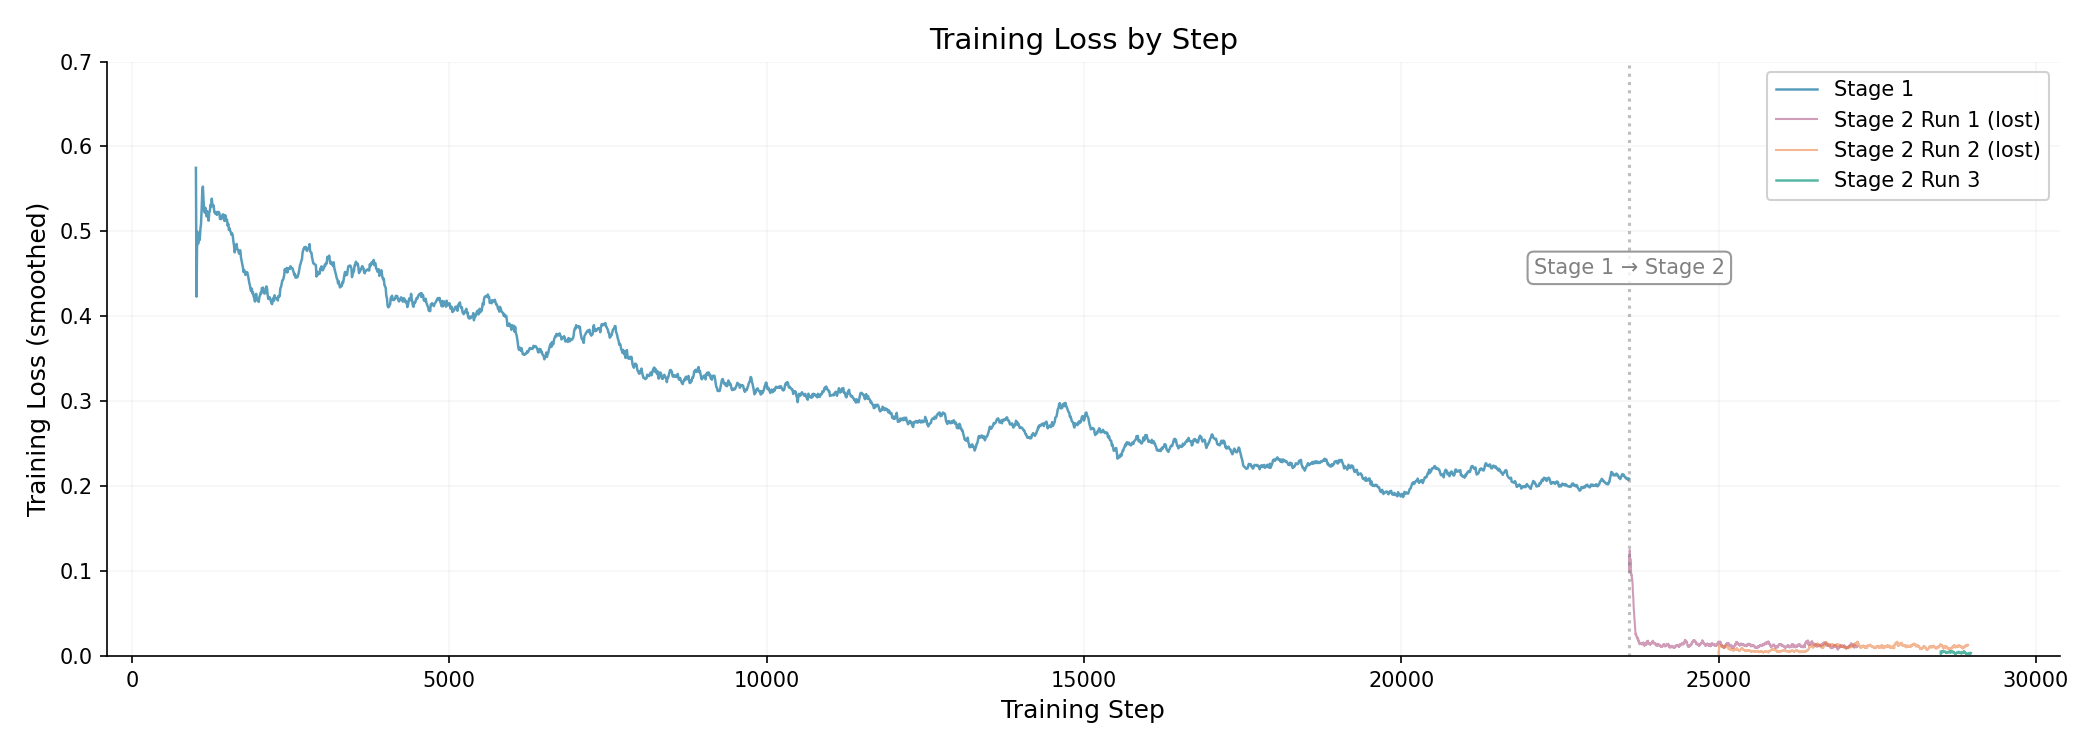
\includegraphics[width=\textwidth]{05_loss_by_step.png}
\caption{Training loss by step across both stages. The stage transition at step 23,594 shows the dramatic shift from visual grounding (loss $\sim$0.13) to multi-turn reasoning (loss $\sim$0.02). Overlapping Stage 2 runs from crash recovery are visible as repeated segments.}
\end{figure}

\subsection{Key Lessons Learned}

\begin{enumerate}
    \item \textbf{Curriculum learning works}: 48\% improvement on visual grounding, 26\% on reasoning
    \item \textbf{More data beats more epochs}: Full dataset showed continued improvement without overfitting
    \item \textbf{Benchmark everything}: Flash Attention wasn't faster on our hardware
    \item \textbf{QLoRA enables accessibility}: 8B model training in $\sim$12GB VRAM
    \item \textbf{Preprocessing is critical}: Garbage in, garbage out
    \item \textbf{Checkpoint frequency is a survival strategy}: Convert save\_steps to wall-clock hours. If $>$ 24h, increase frequency.
    \item \textbf{Design for crashes, not success}: Two OOM crashes during Stage 2, zero during Stage 1. The difference was memory headroom.
    \item \textbf{Log everything to CSV}: When a crash happens at 3 AM, post-hoc analysis of per-step metrics is your only diagnostic tool.
    \item \textbf{Verify checkpoint loading explicitly}: Silent restarts waste hours of compute. Log adapter loading and sanity-check first-step loss.
    \item \textbf{System logs outlive Python logs}: \texttt{journalctl} and \texttt{/var/log/kern.log.1} contain the real crash evidence after a reboot.
    \item \textbf{Monitor your training}: A simple watchdog cron job can detect failures in minutes instead of hours. If you're not monitoring it, you're not running it.
\end{enumerate}

%==========================================
\section{Appendix: Running the Code}
%==========================================

\subsection{Installation}

\begin{lstlisting}[language=bash,caption=Installation commands]
# Clone repository
git clone https://github.com/giricme/vlm-ft.git
cd vlm-ft

# Install dependencies
pip install -e .

# Download data
python -m vlmft.data.download_robovqa --output-dir data/robovqa/raw
\end{lstlisting}

\subsection{Preprocessing}

\begin{lstlisting}[language=bash,caption=Preprocessing commands]
# Preprocess RoboVQA
python -m vlmft.data.preprocess_robovqa \
    --data-dir data/robovqa/raw \
    --output-dir data/robovqa/processed \
    --workers 8

# Verify preprocessing
python -m vlmft.data.preprocess_robovqa \
    --verify \
    --output-dir data/robovqa/processed
\end{lstlisting}

\subsection{Training}

\begin{lstlisting}[language=bash,caption=Training commands]
# Stage 1: Visual Grounding
python -m vlmft.scripts.train --config configs/stage1_full.yaml

# Stage 2: Multi-Turn Reasoning (after Stage 1 completes)
python -m vlmft.scripts.train --config configs/stage2_full.yaml

# Evaluation
python -m vlmft.scripts.eval \
    --checkpoint experiments/stage1/checkpoints/final \
    --config configs/stage1.yaml
\end{lstlisting}

\subsection{Configuration Override}

\begin{lstlisting}[language=bash,caption=Configuration override example]
# Override specific parameters
python -m vlmft.scripts.train \
    --config configs/stage1.yaml \
    data.subset_ratio=0.1 \
    batch_size=4 \
    optimizer.learning_rate=2e-5
\end{lstlisting}

%==========================================
\section{Conclusion}
%==========================================

Fine-tuning Vision-Language Models for robotics is now accessible thanks to QLoRA and curriculum learning. But the gap between ``training works on a small test'' and ``training completes successfully over weeks'' is enormous. The key insights from this project:

\begin{enumerate}
    \item \textbf{Start with foundations}: Visual grounding before complex reasoning
    \item \textbf{Use QLoRA}: Makes large model training feasible
    \item \textbf{Preprocess carefully}: Data quality determines success
    \item \textbf{Validate incrementally}: 10\% runs before full training
    \item \textbf{Engineer for failure}: Aggressive checkpointing, comprehensive logging, explicit verification
    \item \textbf{Know your system tools}: \texttt{dmesg}, \texttt{journalctl}, kernel logs, and thermal monitoring are as important as your training script
\end{enumerate}

The trained model demonstrates strong performance on robotics VQA tasks, with significant improvements from curriculum learning. But equally valuable are the operational lessons: the checkpoint strategy that saved days of compute, the logging that enabled root-cause analysis, and the system debugging that identified memory pressure as the failure mode. These lessons generalize to any long-running training workload.

\vspace{1cm}
\begin{center}
\textit{Code: \url{https://github.com/giricme/vlm-ft}} \\
\textit{Model weights freely available via HuggingFace (links in repo)}
\end{center}

\end{document}
